\documentclass[a4paper,12pt]{article}
\usepackage[a4paper, total={180mm, 272mm}]{geometry}

\usepackage{fontspec}
\setmainfont{ipaexm.ttf}

\graphicspath{{images/}}

\setlength\parindent{4.2em}
\setlength\parskip{0em}
\renewcommand{\baselinestretch}{1.247}

\begin{document}

\thispagestyle{empty}

\Large
\noindent \\
Radial Blur Ino\medskip
\par
\normalsize
放射方向に平均値ぼかしを行ないます。\par
方向にねじれを加えることも可能です(処理時間がよりかかります)。\\
\par
初めに、指定あれば Alpha チャンネルに対して処理します。\par
次に、Alpha チャンネルがゼロでないピクセルの RGB を処理します。\par
Alpha チャンネルに処理をしないときは、RGB 画像の変化を Alpha 値\par
でマスクします。よって、滑らかなエッジは滑らかなままです。\\
\\
--- \ 入力 \ ---\\
Source\par
処理をする画像を接続します。\\
Reference\par
Pixel 毎に効果の強弱をつけるための参照画像を接続します。\\
\\
--- \ 設定 \ ---\\
Center\par
放射の中心位置を指定します。\par
原点は処理をする画像の中心です。カメラの注視点ではありません。\par
単位はミリメートルです。\par
初期値は"0.0 0.0"で原点位置が中心です。\\
\\
Radius\par
中心からぼかさない範囲を指定します。\par
単位はミリメートルです。\par
0以上の値を入力します。\par
初期値は0で全体にぼかします。\\
\\
Blur\par
ぼかしの強さを調整をします。\par
ぼかしの強さは、Center から各 Pixel までの長さで決まります。\par
計算式は、Center から各 Pixel の距離を Pixel\_Len とすると、\par
(Pixel\_Len - Radius) * (Blur / 100)\par
となります。\par
最小は0でこのときは何もしません。最大は100です。\par
初期値は1です。

\newpage

\thispagestyle{empty}

\ \vspace{-0.2em}
\par
\noindent Twist\par
ひねりを加えます。\par
このひねりは Center から基準距離までを何度ひねるかで指定します。\par
基準距離は、結果画像の上下高の半分の長さです。\par
最小は0でひねりません。最大は180です。\\
\\
Alpha Rendering\par
ON で Alpha にも処理をします。\par
OFF のときは、Alpha に処理しませんが、\par
RGB 値の変化を Alpha 値でマスクします。\par
初期値は ON です。\\
\\
Anti Alias\par
ジャギーをなくすためにアンチエイリアスを加えた処理を行います。\par
結果はなめらかになりますが時間がかかります。\par
初期値は OFF です。\par
<処理時間参考例>\par
Width=2176 Height=1236 Center=0,0 Radius=0 Blur=3 Alpha=ON\par
Shrink=1\par
\noindent \hskip 7em Twist=0\par
\noindent \hskip 10.5em Anti Alias=OFF 約7sec\par
\noindent \hskip 10.5em Anti Alias=ON \, 約32sec\par
\noindent \hskip 7em Twist=1-180\par
\noindent \hskip 10.5em Anti Alias=OFF 約19sec\par
\noindent \hskip 10.5em Anti Alias=ON \, 約780sec\par
Shrink=3\par
\noindent \hskip 7em Twist=0\par
\noindent \hskip 10.5em Anti Alias=OFF 約3sec\par
\noindent \hskip 10.5em Anti Alias=ON \, 約4sec\par
\noindent \hskip 7em Twist=1-180\par
\noindent \hskip 10.5em Anti Alias=OFF 約4sec\par
\noindent \hskip 10.5em Anti Alias=ON \, 約34sec\\
\\
Reference\par
Pixel 毎に効果の強弱をつけるための参照画像の値の取り方を選択します。\par
入力の"Reference"に画像を接続し、\par
Red/Green/Blue/Alpha/Luminance/Nothing から選びます。\par
この効果をつけたくないときは Nothing を選ぶか、接続を切ります。\par
初期値は Red です。

\newpage

\thispagestyle{empty}

\ \vspace{-0.2em}
\par
\noindent Radial Blur \ \ 参考例

\large
\noindent \begin{picture}(0,0)
\put(170.5,-144.5){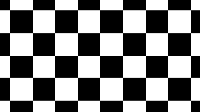
\includegraphics[width=13.3em]{RadialBlurInoOriginalImage}}
\put(92.5,-343){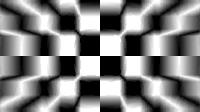
\includegraphics[width=13.3em]{RadialBlurInoRadialBlur30AAOFF}}
\put(314.5,-343){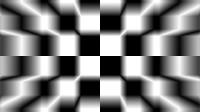
\includegraphics[width=13.3em]{RadialBlurInoRadialBlur30AAON}}
\put(92.5,-486){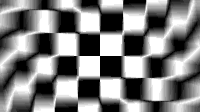
\includegraphics[width=13.3em]{RadialBlurInoTwistBlur20Twist45AAOFF}}
\put(314.5,-486){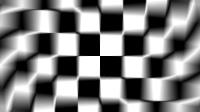
\includegraphics[width=13.3em]{RadialBlurInoTwistBlur20Twist45AAON}}
\put(26,-50){\normalsize{元画像}}
\put(26,-67){\normalsize{(200x112pixel)}}
\put(89,-221){\normalsize{Anti Alias \ \ OFF}}
\put(311,-221){\normalsize{Anti Alias \ \ ON}}
\put(26,-249){\normalsize{Radial}}
\put(26,-267){\normalsize{(Blur 30)}}
\put(26,-382){\normalsize{Twist}}
\put(26,-400){\normalsize{(Blur 20}}
\put(32,-418){\normalsize{Twist 45)}}
\end{picture}\\[12.65em]

\end{document}